\documentclass[herrin-thesis.tex]{subfiles}
\begin{document}

\chapter{The EXO-200 Detector}
\label{ch:detector}

\section{Overview}


\section{A Xenon Detector}
Xenon has many properties that make it useful for a double beta decay experiment:
\begin{itemize}
\item First and foremost, xenon can serve as both as the source and detector of double beta decay events. This minimizes the other materials needed to build the detector that might be sources of radioactive backgrounds. Electrons from the double beta decay do not have to pass through other media before reaching the detector, allowing fewer energy losses and better energy resolution.
\item The Q value for \xenon{136} decays is is \SI{2457.8}{\keV}\cite{Redshaw:2007cr}, which is higher that most \(\gamma\) rays from common radioactive nuclides. \isotope{208}{Tl}, which occurs on the thorium chain and emits a \SI{2615}{\keV}gamma ray is the notable exception. \(\gamma\) rays with higher energies than the Q value can potentially deposit part of their energy in the detector before scattering out, creating an event with energy close to the Q value.
\item The natural abundance of \xenon{136} is 8.9\%. Furthermore, xenon is a gas at standard temperatures and pressures, making it simple to process and enrich in \xenon{136} using ultracentrifugation.
\item Xenon is a nobel element, and so it is relatively easy to purify of all chemically active contaminants. Furthermore, this purification can be done continuously by recirculating the xenon.
\item The isotopes formed in xenon by cosmogenic activation are short-lived, so the xenon only needs a short period underground and a chemical purification before it is ready to be used.
\item Xenon can be easily reused and transferred between experiments. This allows the opportunity to use xenon in complimentary or novel detector designs. Smaller experiments can help amortize the cost of larger experiments.
\item The barium daughter ion could potentially be tagged, reducing backgrounds immensely. (This technique, however, is not used in EXO-200.)
\end{itemize}

As the name suggests, EXO-200 makes use of \SI{200}{\kg} of xenon, enriched to 80.6\% in \xenon{136} with clean centrifuges at several laboratories in Russia. Of the remaining fraction of the xenon, isotope 134 comprises 19.1\%, and lighter natural elements are present in trace amounts. \isotope{85}{Kr} is present at \SI[per-mode=symbol]{25.5\pm3.0d-12}{\g\per\g}\cite{Dobi:2012nx}. This low contamination and low Q value mean it is not problematic for EXO-200.

\section{Time Projection Chamber}
EXO-200 uses xenon in the liquid phase to make a Time Projection Chamber (TPC). When a process deposits energy in liquid xenon, it creates both scintillation light and ionization. Avalanche PhotoDiodes (APDs) detect the scintillation nearly instantaneously. The ionization, meanwhile, drifts in an applied electric field to crossed wire planes, where it induces a signal in one plane (the ``v'' wires) and is collected on the other plane (the ``u'' wires). \Cref{fig:detector_tpc_cartoon} provides a schematic of the TPC concept for EXO-200. The crossed wire grids provide a 2D projection of the event, while the time between the scintillation signal and the ionization signal provides a \(z\) coordinate. The EXO-200 chamber is actually divided into two separate TPCs by a cathode, biased to \SI{-8.0}{\kV}, producing a drift field of \SI{374}{\V\per\cm}

\begin{figure}
\centering
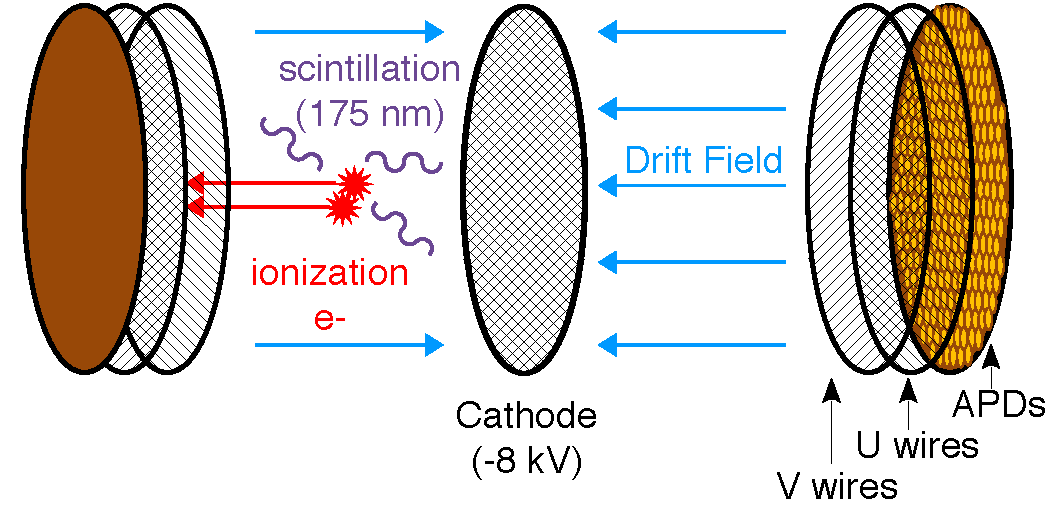
\includegraphics[width=0.6\textwidth]{./figures/tpc_schematic.pdf}
\caption[A schematic of a TPC]{A schematic of the TPC concept for EXO-200.}
\label{fig:detector_tpc_cartoon}
\end{figure}

The use of a liquid-phase TPC has several advantages for a low-background experiment. The xenon at the outer edges of the detector, outside of the active region, provides modest self shielding against \(\gamma\) rays. The scintillation and the ionization signals can be combined to give good energy resolution\cite{Conti:2003tg}\cite{Aprile:2007hc}. \(\gamma\) ray backgrounds near the Q value of \xenon{136} most often deposit their energy via Compton scattering or electron-positron pair production. These processes create spatially-separated ionization signals, which can then be distinguished from double beta decays, which deposit their energy at a single location in a small volume.

\section{Calibration}

\begin{figure}[htb]
\centering
\begin{subfigure}[c]{0.33\linewidth}
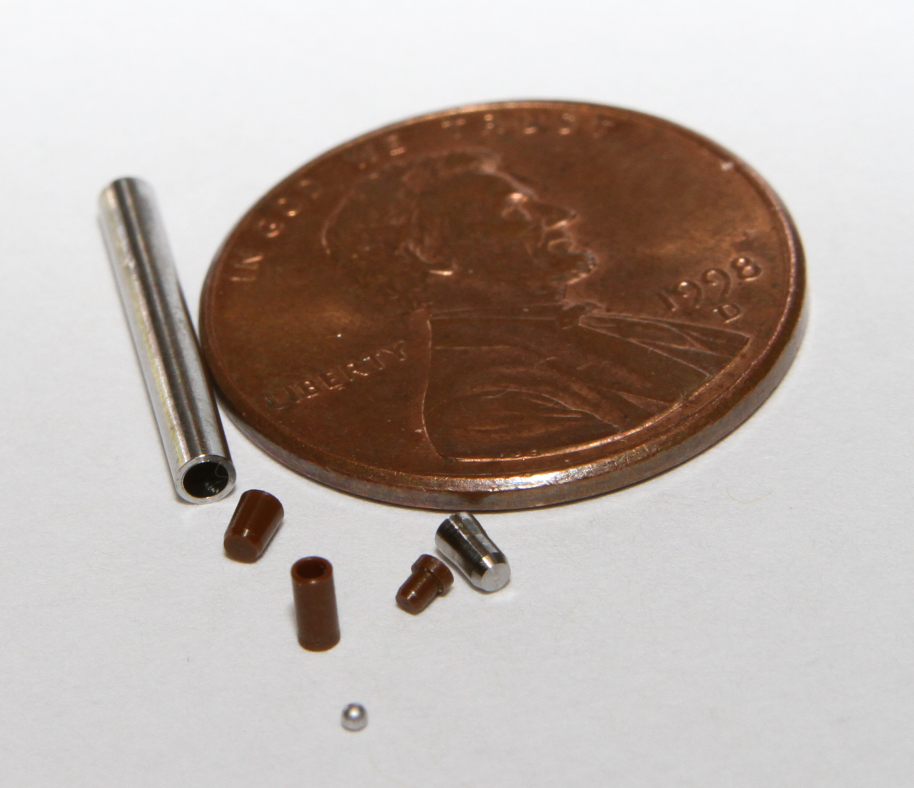
\includegraphics[width=\textwidth]{./photos/source_capsule.png}
\end{subfigure}\hspace{0.05\linewidth}\hfill%
\begin{subfigure}[c]{0.60\linewidth}
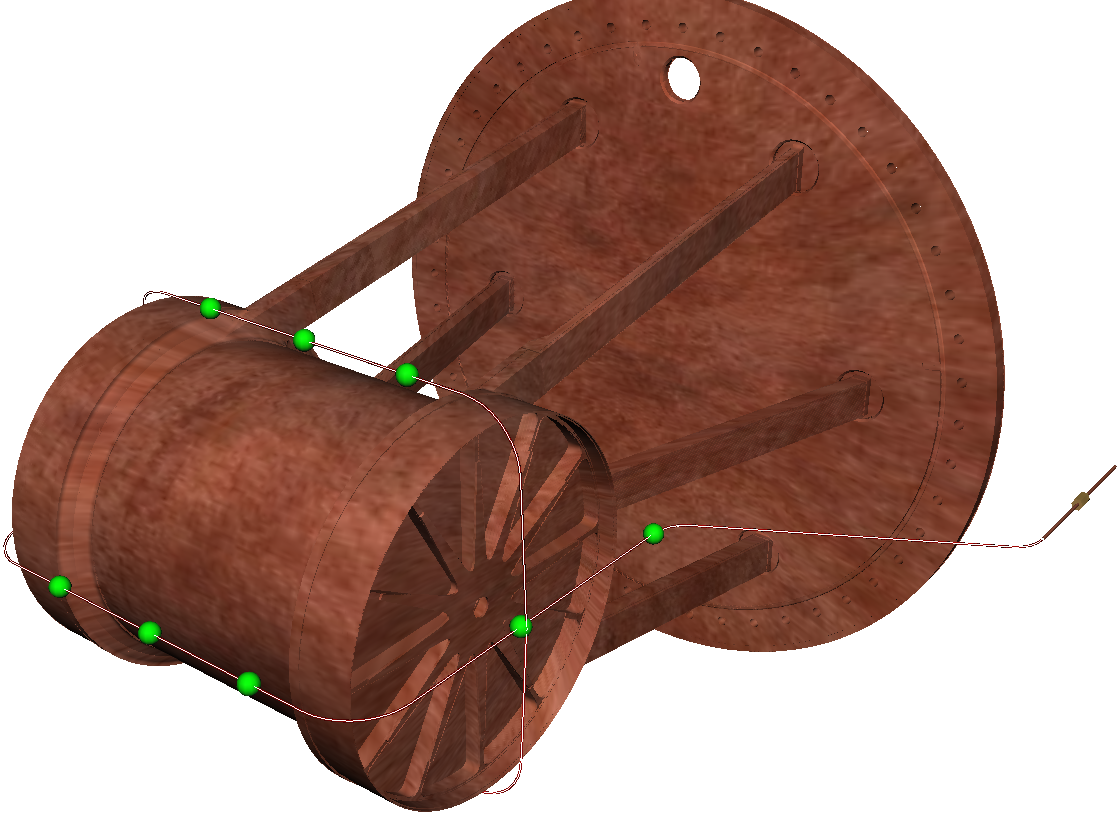
\includegraphics[width=\textwidth]{./photos/calibration_tubing_cropped.png}
\end{subfigure}
\caption[The Calibration System]{To calibrate the detector, a tiny source capsules (left) containing a radioisotope can be deployed to many positions just outside the detector through a guide tube system (right).}
\label{fig:detector_calibration}
\end{figure}

\section{WIPP}

\begin{figure}[htb]
\centering
\begin{subfigure}[c]{0.30\linewidth}
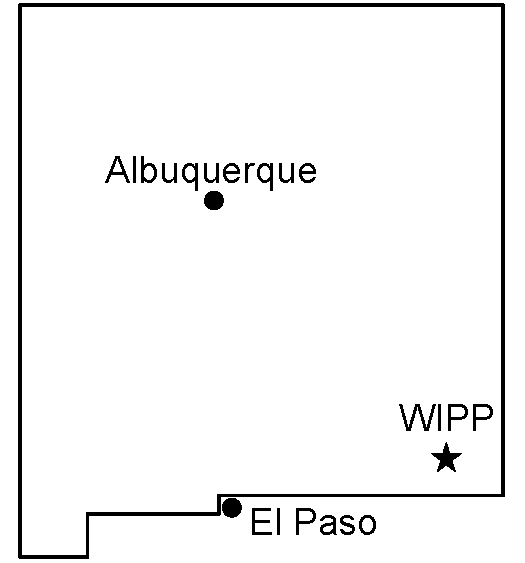
\includegraphics[width=\textwidth]{./figures/wipp_map.pdf}
\end{subfigure}\hspace{0.05\linewidth}\hfill%
\begin{subfigure}[c]{0.60\linewidth}
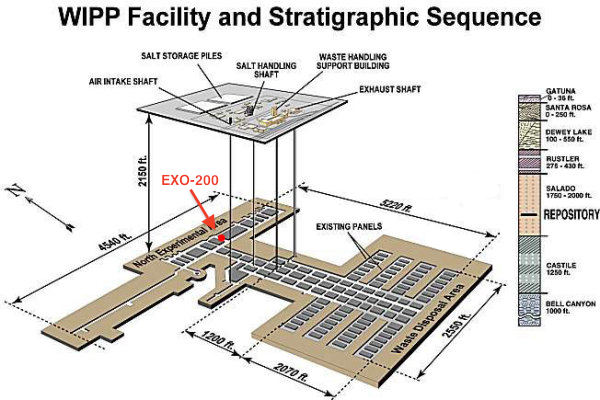
\includegraphics[width=\textwidth]{./photos/wipp_site_annotated.png}
\end{subfigure}
\caption[The WIPP Site]{The left shows the location of the WIPP site on a map of New Mexico. The right shows a detailed view of the WIPP site. EXO-200 is located in the North Experimental Area, approximately \SI{655}{\m} underground.}
\label{fig:detector_wipp}
\end{figure}

In order to shield from cosmic rays that are a potential background, EXO-200 is located \(\sim\)~\SI{655}{\m} underground at the Department of Energy's Waste Isolation Pilot Plant (WIPP) in southeastern New Mexico. WIPP is a salt mine, and its primary purpose is the permanent disposal of transuranic waste. The north end of the mine, far from the waste, serves as a suitable site for low-background experiments.

The rock overburden provides \SI{1450}{\hecto\g\per\square\cm} shielding from cosmic rays (see \cref{ch:muons}), and the salt walls are naturally low in radionuclides. Direct counting finds a contamination of \SI[per-mode=symbol]{27\pm2d-9}{\g\per\g} of \isotope{238}{U}, \SI[per-mode=symbol]{66\pm2d-9}{\g\per\g} of \isotope{232}{Th}, and \SI[per-mode=symbol]{124\pm2}{\g\per\g} of \isotope{40}{K}\todo{Find a source for this besides Russell's thesis.}. Little radon emanates from the walls, such that radon levels are similar to those found at the surface.


\end{document}
